\documentclass[aspectratio=169,11pt]{beamer}

% ==================================================
% Talk version of asa-paper/ms.tex
% Story principle: every beat is connected by "BUT" or "THEREFORE"
% ==================================================

\usetheme{metropolis}
\usecolortheme{crane}

% --- Basic packages ---
\usepackage{graphicx}
\usepackage{booktabs}
\usepackage{amsmath,amssymb,mathtools}
\usepackage{tabularx}
\usepackage{ragged2e}
\usepackage[table]{xcolor}
\usepackage{hyperref}

% --- TikZ ---
\usepackage{tikz}
\usetikzlibrary{arrows.meta,calc,positioning,fit,shapes.geometric,shapes.misc,backgrounds}

% --- Bibliography (shared with paper) ---
\usepackage[natbib=true,minnames=1,maxnames=3,backend=biber,style=authoryear-luh-ipw]{biblatex}
\addbibresource{../../Paper/mybib.bib}

% --- Figures / generated macros ---
\graphicspath{{./../../Figures/}}
\newcommand{\LLMOverallAccAllpolparty}{0.751}
\newcommand{\LLMOverallAccHighpolparty}{0.860}
\newcommand{\LLMMeanLowConfpolparty}{0.250}
\newcommand{\LLMMedianLowConfpolparty}{0.250}
\newcommand{\LLMMeanAccByCountryHighpolparty}{0.879}
\newcommand{\LLMMeanBaselineByCountrypolparty}{0.536}
\newcommand{\LLMMeanDeltaByCountrypolparty}{0.343}
\newcommand{\LLMMinDeltaByCountrypolparty}{-0.602}
\newcommand{\LLMMaxDeltaByCountrypolparty}{0.761}
\newcommand{\LLMMinDeltaCountrypolparty}{Gambia}
\newcommand{\LLMMaxDeltaCountrypolparty}{Finland}
\newcommand{\LLMMeanAccSmallGroupspolparty}{0.692}
\newcommand{\LLMMeanAccLargeGroupspolparty}{0.820}
\newcommand{\LLMNumCountriespolparty}{114}
\newcommand{\LLMNumInstancespolparty}{34,618}
\newcommand{\LLMNumClassespolparty}{1,209}
\newcommand{\LLMNumPredictionsGainedpolparty}{12,898}
\newcommand{\LLMNumPredictionsGainedPercentpolparty}{20.8}
\newcommand{\LLMRelaxedChangedPctpolparty}{2.5}


% --- Metropolis tweaks ---
\metroset{progressbar=frametitle,numbering=fraction}
\setbeamertemplate{footline}{}
\setbeamertemplate{caption}[numbered]
\setbeamertemplate{itemize items}[circle]

\definecolor{RowShade}{gray}{0.95}
\newcolumntype{Y}{>{\RaggedRight\arraybackslash}X}

% --- Title block ---
\title{A Verifiable Search Agent (ASA) for Political Elite Research}
\author{More at \texttt{connorjerzak.com}}
\date{}

\begin{document}

% --------------------------------------------------
% Title slide (manual to avoid metropolis title-page overflow)
\begin{frame}[plain,noframenumbering]
  \vspace{1.2em}
  {\LARGE\bfseries \inserttitle\par}
  \vspace{0.8em}
  {\large \insertauthor\par}
\end{frame}
% --------------------------------------------------

\begin{frame}[standout]
Elite attribute labels are \textbf{measurements}.\\[0.4em]
\normalsize
\textbf{Therefore} they must be auditable, comparable, and time-defined.
\end{frame}

\begin{frame}{LLMs show potential}{}
  \Large
But they break three dataset requirements: 
\begin{columns}[T,onlytextwidth]
  \column{0.33\textwidth}
  \textbf{Non-verifiable}\\[-2pt]
  \normalsize
  No durable evidence trail (queries, snippets, URLs, timestamps).

  \column{0.33\textwidth}
  \textbf{Non-comparable}\\[-2pt]
  \normalsize
  Open-world labels drift across countries and years (synonyms, translations, rebrands).

  \column{0.33\textwidth}
  \textbf{Temporal leakage}\\[-2pt]
  \normalsize
	  Coding year \(t\) using post-\(t\) sources contaminates ``baseline'' covariates.
	\end{columns}

	\vspace{0.6em}
	\hfill\scriptsize{\parencite{ji2023hallucination}}
\end{frame}

\begin{frame}{AI Search Agents Overcome Limitations}{}
  \large
\begin{columns}[T,onlytextwidth]
  \column{0.33\textwidth}
  \begin{block}{Verifiable}
    Evidence-first outputs\\
    + explicit citations\\
    + full trace archive
    + low tool cost vs. APIs 
  \end{block}

  \column{0.33\textwidth}
  \begin{block}{Comparable}
    Closed codebooks\\
    + conservative normalization\\
    + no new labels
  \end{block}

  \column{0.33\textwidth}
  \begin{block}{Temporal leakage}
    ``As-of'' constraints\\
    + date checks \\
    + temporally constrained search
	  \end{block}
	\end{columns}

	\vspace{0.6em}
	\hfill\scriptsize{\parencite{nakano2021webgpt,yao2022react}}
\end{frame}

\begin{frame}[standout]
\textbf{} Treat web retrieval as a\\
\textbf{governed, auditable measurement instrument}.
\end{frame}

\begin{frame}{ASA in one picture}{Inputs and outputs are verifiable by construction}
\vspace{-0.3em}
\centering
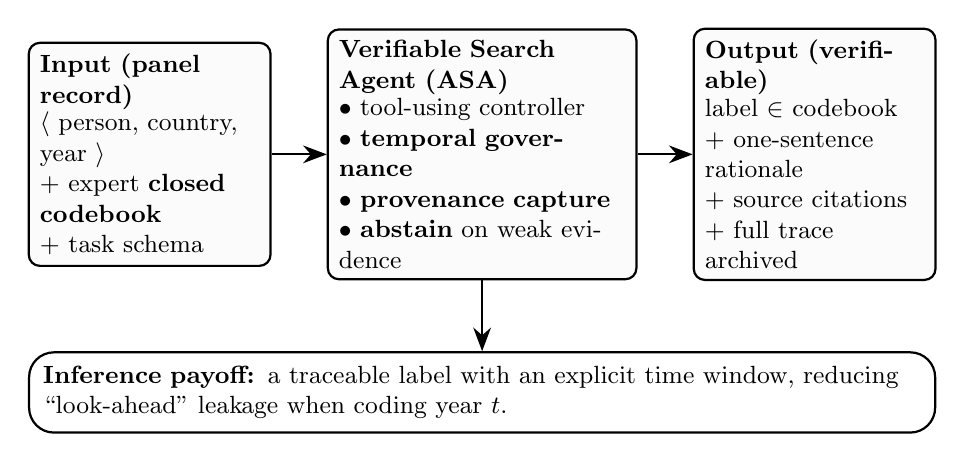
\begin{tikzpicture}[
  font=\small,
  node distance=9mm and 7mm,
  box/.style={rounded corners, draw=black, thick, fill=gray!3, inner sep=4pt, align=left},
  pill/.style={rounded corners=9pt, draw=black, thick, fill=white, inner sep=5pt, align=left},
  arr/.style={-{Stealth[length=3mm]}, thick},
]
  \node[box, text width=0.23\linewidth] (input) {
    \textbf{Input (panel record)}\\[-1pt]
    \(\langle\) person, country, year \(\rangle\)\\
    + expert \textbf{closed codebook}\\
    + task schema
  };

  \node[box, right=of input, text width=0.30\linewidth] (agent) {
    \textbf{Verifiable Search Agent (ASA)}\\[-1pt]
    \(\bullet\) tool-using controller\\
    \(\bullet\) \textbf{temporal governance}\\
    \(\bullet\) \textbf{provenance capture}\\
    \(\bullet\) \textbf{abstain} on weak evidence
  };

  \node[box, right=of agent, text width=0.23\linewidth] (output) {
    \textbf{Output (verifiable)}\\[-1pt]
    label \(\in\) codebook\\
    + one-sentence rationale\\
    + source citations\\
    + full trace archived
  };

  \draw[arr] (input) -- (agent);
  \draw[arr] (agent) -- (output);

  \node[pill, below=9mm of agent, text width=0.92\linewidth] (why) {
    \textbf{Inference payoff:} a traceable label with an explicit time window, reducing ``look-ahead'' leakage when coding year \(t\).
  };
  \draw[arr] (agent.south) -- (why.north);
\end{tikzpicture}
\end{frame}

\begin{frame}{Commercial search tools vs. asa}{But dataset creation requires scientific control}
\vspace{-0.5em}
\begin{table}
  \centering
  \renewcommand{\arraystretch}{1.5} % Adds vertical padding for a clean look without booktabs/shading
  \begin{tabular}{p{0.22\textwidth} p{0.34\textwidth} p{0.34\textwidth}}
    \hline\hline
    \textbf{Requirement} & \textbf{Commercial Grounded LLMs}
%                           \newline {\footnotesize(e.g., Gemini / ChatGPT search)}
    & \textbf{ASA Protocol} \\
    \hline
    \textbf{Provenance} & Opaque query generation; ephemeral links. & Full trace of all queries, raw snippets, URLs, tool calls. \\
    \textbf{Temporal Bounds} & Biased toward the live/current web. & Strict ``as-of'' date constraints, checks. \\
%    \textbf{Comparability} & Open-ended text that drifts across sessions and languages. & Forced alignment to expert, country-specific closed codebooks. \\
    \textbf{Cost \& Control} & High search cost (\$10 per 1k queries). & Modular, low-cost tool routing. \\
    \hline\hline
  \end{tabular}
\end{table}

\vspace{0.8em}
\large
\textbf{Therefore:} ASA decouples the search execution from the reasoning step, lowering costs while guaranteeing an auditable evidence trail.
\end{frame}

\begin{frame}{How ASA works}{A short, budgeted search session with an auditable trace store}
\vspace{-0.5em}
\centering
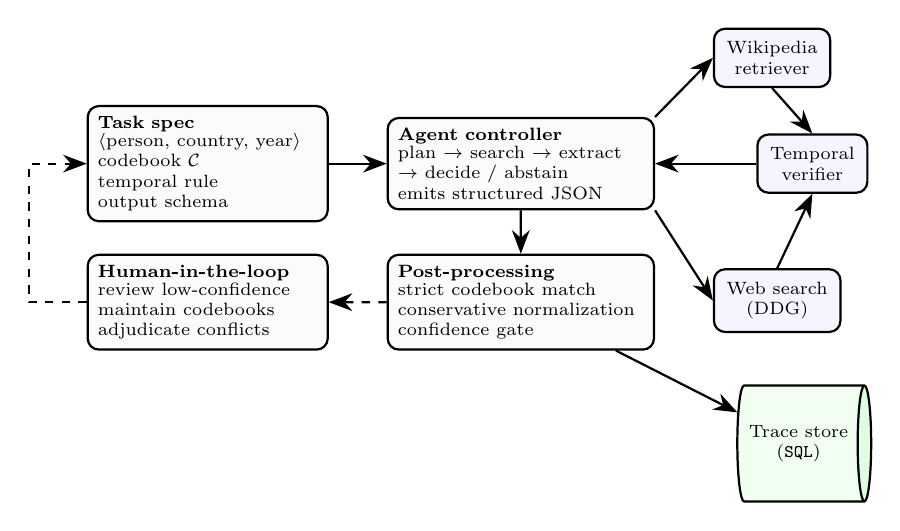
\begin{tikzpicture}[
  scale=0.92,
  transform shape,
  font=\scriptsize,
  node distance=6mm and 8mm,
  comp/.style={rounded corners, draw=black, thick, fill=gray!3, inner sep=4pt, align=left},
  tool/.style={rounded corners, draw=black, thick, fill=blue!4, inner sep=5pt, align=center},
  store/.style={cylinder, cylinder uses custom fill, cylinder body fill=green!6, cylinder end fill=green!12, draw=black, thick, aspect=0.25, minimum height=18mm, minimum width=16mm, align=center},
  arr/.style={-{Stealth[length=3mm]}, thick},
  loop/.style={-{Stealth[length=3mm]}, thick, dashed},
]
  \node[comp, text width=0.25\linewidth] (spec) {
    \textbf{Task spec}\\[-1pt]
    \(\langle\)person, country, year\(\rangle\)\\
    codebook \(\mathcal{C}\)\\
    temporal rule\\
    output schema
  };

  \node[comp, right=of spec, text width=0.28\linewidth] (graph) {
    \textbf{Agent controller}\\[-1pt]
    plan \(\rightarrow\) search \(\rightarrow\) extract\\
    \(\rightarrow\) decide / abstain\\
    emits structured JSON
  };

  \node[tool, above right=4mm and 8mm of graph] (wiki) {Wikipedia\\retriever};
  \node[tool, below right=8mm and 8mm of graph] (web) {Web search\\(DDG)};
  \node[tool, right=14mm of graph] (time) {Temporal\\verifier};

  \node[comp, below=of graph, text width=0.28\linewidth] (post) {
    \textbf{Post-processing}\\[-1pt]
    strict codebook match\\
    conservative normalization\\
    confidence gate
  };

  \node[store, below right=5mm and 12mm of post] (db) {Trace store\\(\texttt{SQL})};

  \node[comp, left=of post, text width=0.25\linewidth] (human) {
    \textbf{Human-in-the-loop}\\[-1pt]
    review low-confidence\\
    maintain codebooks\\
    adjudicate conflicts
  };

  \draw[arr] (spec) -- (graph);
  \draw[arr] (graph) -- (post);
  \draw[arr] (post) -- (db);

  \draw[arr] (graph.north east) -- (wiki.west);
  \draw[arr] (graph.south east) -- (web.west);
  \draw[arr] (wiki.south) -- (time.north);
  \draw[arr] (web.north) -- (time.south);
  \draw[arr] (time.west) -- ([xshift=0mm]graph.east);

  \draw[loop] (post.west) -- (human.east);
  \draw[loop] (human.west) -| ([xshift=-8mm]spec.west) -- (spec.west);
\end{tikzpicture}
\end{frame}

\begin{frame}{Temporal governance}{But without time rules, ``accuracy'' can be look-ahead leakage}
\large
\begin{columns}[T,onlytextwidth]
  \column{0.58\textwidth}
  \begin{itemize}
    \item Target: attribute at year \(t\) (pre-period state).
    \item Common failure: use a source updated long after \(t\), which summarizes later events.
    \item \textbf{Result:} your ``baseline'' covariate may encode post-\(t\) outcomes (party switches, coalitions).
  \end{itemize}

  \column{0.42\textwidth}
  \centering
  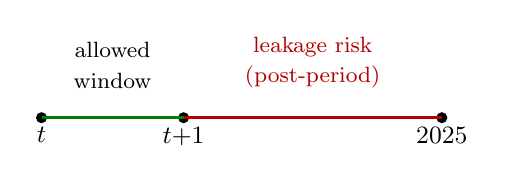
\begin{tikzpicture}[x=0.82cm,y=1cm,>=Stealth,font=\small]
    \draw[thick] (0,0) -- (6.2,0);
    \node[below] at (0,0) {\(t\)};
    \node[below] at (2.2,0) {\(t{+}1\)};
    \node[below] at (6.2,0) {2025};
    \fill (0,0) circle (2pt);
    \fill (2.2,0) circle (2pt);
    \fill (6.2,0) circle (2pt);
    \draw[very thick,green!50!black] (0,0) -- (2.2,0);
    \node[above,align=center] at (1.1,0.25) {\footnotesize allowed\\\footnotesize window};
    \draw[very thick,red!70!black] (2.2,0) -- (6.2,0);
    \node[above,align=center,text=red!70!black] at (4.2,0.25) {\footnotesize leakage risk\\\footnotesize (post-period)};
	  \end{tikzpicture}
	\end{columns}

	\vspace{0.4em}
	\hfill\scriptsize{\parencite{kaufman2012leakage,montgomery2018conditioning}}
\end{frame}

\begin{frame}{Temporal governance}{Therefore: ``as-of'' constraints + date checks + abstention}
\large
\begin{itemize}
  \item Each run has an explicit ``as-of'' rule (e.g., sources published before \(t{+}1\)).
  \item When feasible: extract publication dates and enforce the cut strictly.
  \item When not feasible: warn and \textbf{abstain} rather than silently rely on post-period material.
  \item Full trace (including timestamps) is stored for later audit and alternative inclusion rules.
\end{itemize}
\end{frame}

\begin{frame}{Case study: party affiliation labeling}{A verifiable attribute with an expert closed codebook}
\large
\begin{itemize}
  \item Task: label party affiliation for \textbf{\LLMNumInstancespolparty{}} leader--records across \textbf{\LLMNumCountriespolparty{}} countries.
  \item Closed world: \textbf{\LLMNumClassespolparty{}} expert party labels (country-specific codebooks).
  \item Agent outputs: label \(\in\) codebook + one-sentence rationale + citations + trace; otherwise abstain.
  \item Evaluation: score \textbf{high-confidence} predictions against expert codings.
\end{itemize}
\end{frame}

\begin{frame}{Results}{Therefore: high-confidence accuracy \LLMOverallAccHighpolparty{} with more usable coverage}
\vspace{-0.2em}
\begin{columns}[T,onlytextwidth]
  \column{0.70\textwidth}
  \centering
  \includegraphics[width=\linewidth]{AgentHist.pdf}

  \column{0.30\textwidth}
  \large
  \begin{itemize}
    \item \textbf{Accuracy (high-conf):} \LLMOverallAccHighpolparty{}
    \item \textbf{Coverage gained:} +\LLMNumPredictionsGainedPercentpolparty{}\%\\(\LLMNumPredictionsGainedpolparty{} new labels)
    \item \textbf{Withheld (low-conf):} \LLMMeanLowConfpolparty{} on average
  \end{itemize}
\end{columns}
\end{frame}

\begin{frame}{Where performance varies}{But heterogeneity is real (time, region, and evidence quality)}
\vspace{-0.3em}
\centering
\includegraphics[width=0.62\linewidth]{AgentOverTime.pdf}
\hfill
\includegraphics[width=0.35\linewidth]{AgentRegionBox.pdf}

\vspace{0.8em}
\large
\begin{itemize}
  \item Earlier years and sparse web records increase abstention and error risk.
  \item Name ambiguity and missing publication dates are recurring failure modes.
\end{itemize}
\end{frame}

\begin{frame}[fragile]{What ``verifiable'' looks like}{Therefore: every label ships with inspectable evidence and a trace}
\scriptsize
\begin{columns}[T,onlytextwidth]
  \column{0.55\textwidth}
  \textbf{Structured output (example)}
\begin{verbatim}
{
  "label": "Party X",
  "confidence": "high",
  "rationale": "… (with citations)",
  "sources": [
    {"url": "...", "date": "..."},
    {"url": "...", "date": "..."}
  ]
}
\end{verbatim}

  \column{0.45\textwidth}
  \textbf{Trace store enables}
  \begin{itemize}
    \item audit any label quickly
    \item replicate and re-filter outputs
    \item route uncertain cases to humans
  \end{itemize}
\end{columns}
\end{frame}

\begin{frame}[standout]
\textbf{Takeaway:} Verifiable agents turn LLM+web retrieval\\
into \textbf{replicable instruments} for dataset construction.
\end{frame}

\appendix
\begin{frame}[allowframebreaks,noframenumbering]{References}
  \scriptsize
  \printbibliography
\end{frame}

\end{document}
